\begin{figure}[t]
\vspace*{5pt}

\center
%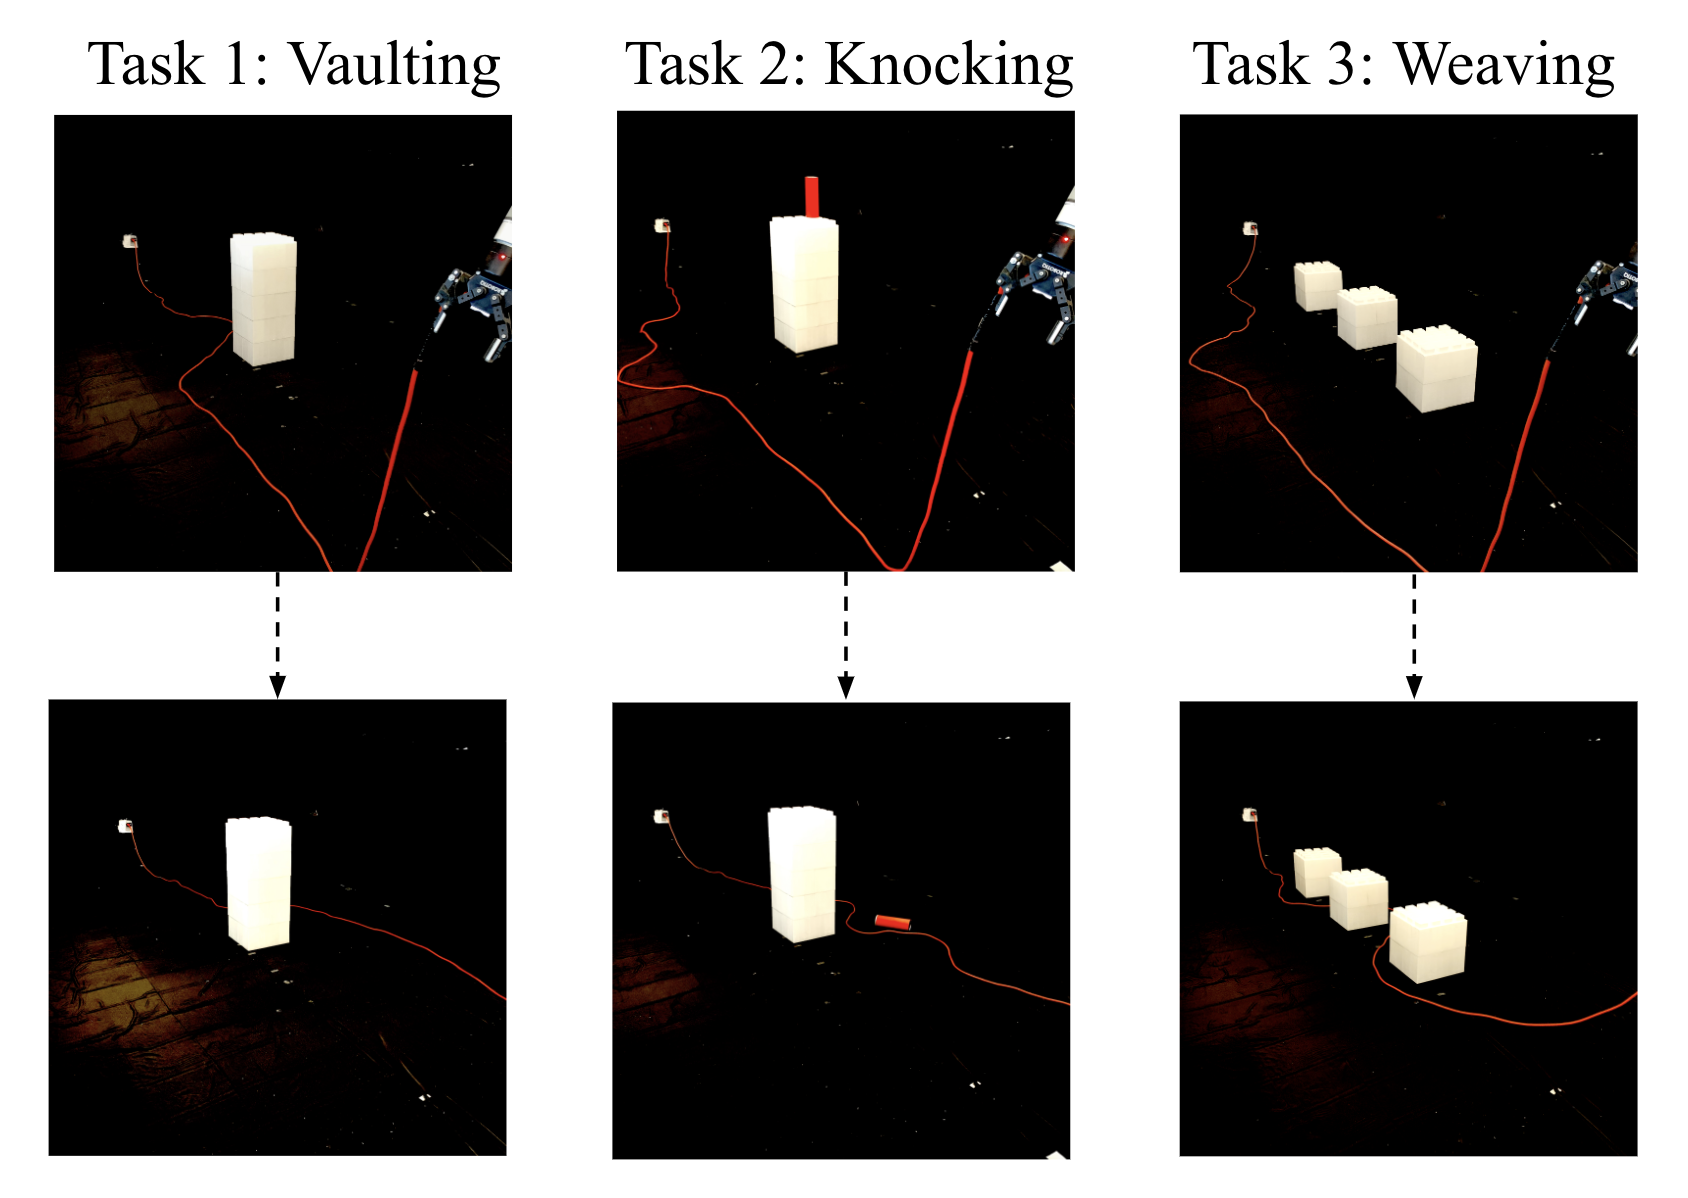
\includegraphics[width=0.48\textwidth]{figures/teaser1.png}
\begin{tikzpicture}[
every node/.style={outer sep=0,node distance=0pt,inner sep=0},
arr/.style={-latex,line width=1pt}]
% IEEE conference format: column width = 3.4in = 244.8pt
% 3 pictures * 80pt = 240pt
% (244.8 - 240)/2 = 4.8/2 = 2.4pt = spacing between pictures
% \node [options] (name) {LaTex Contents of Node};


% \draw [-Triangle,thick] (from_name) -- (to_name); 
% "-Latex" and "-triangle" are arrow types
\node (vs) {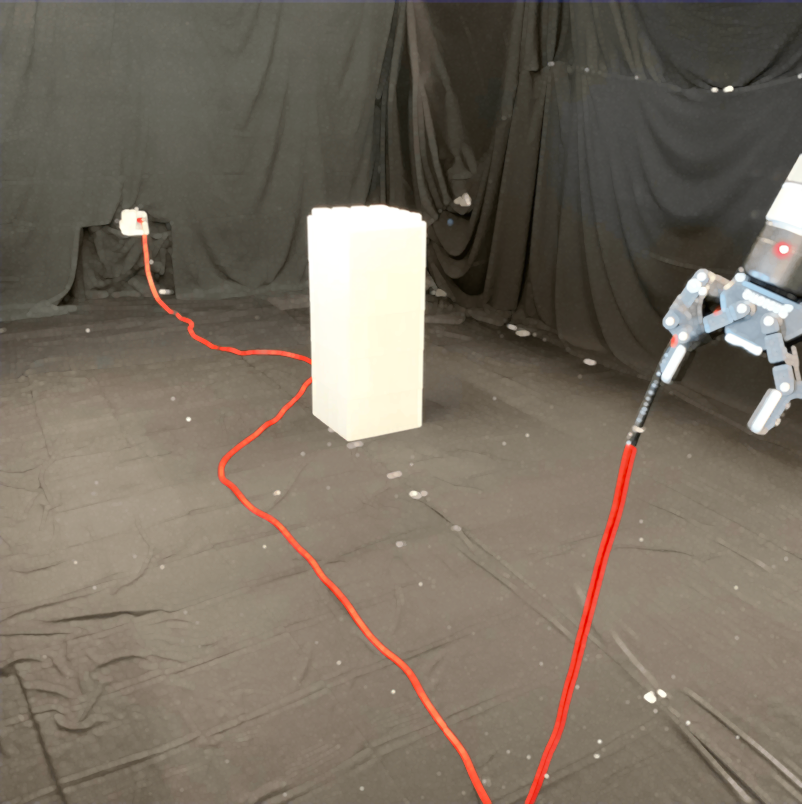
\includegraphics[width=80pt]{figures/teaser_vaulting_start.png}};
\node [right=2.4pt of vs] (ks) {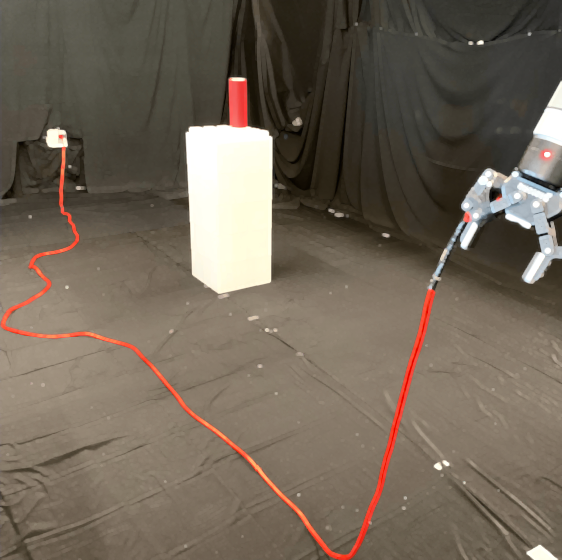
\includegraphics[width=80pt]{figures/teaser_knocking_start.png}};
\node [right=2.4pt of ks] (ws) {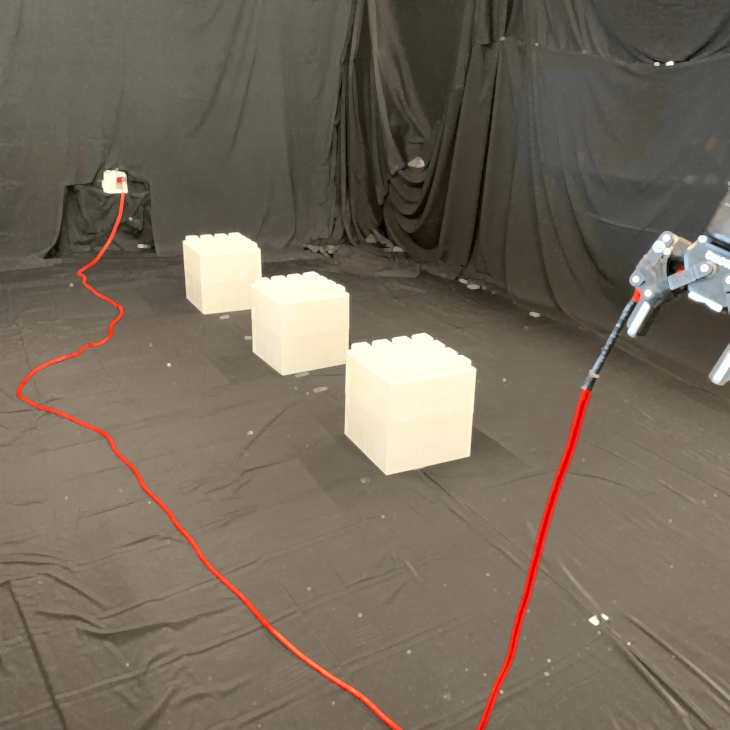
\includegraphics[width=80pt]{figures/teaser_weaving_start.png}};
\node [below=12pt of vs] (ve) {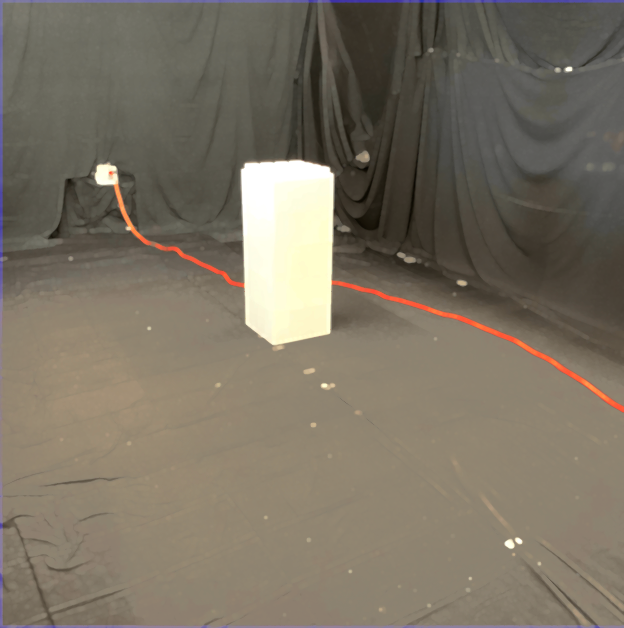
\includegraphics[width=80pt]{figures/teaser_vaulting_end.png}};
\node [below=12pt of ks] (ke) {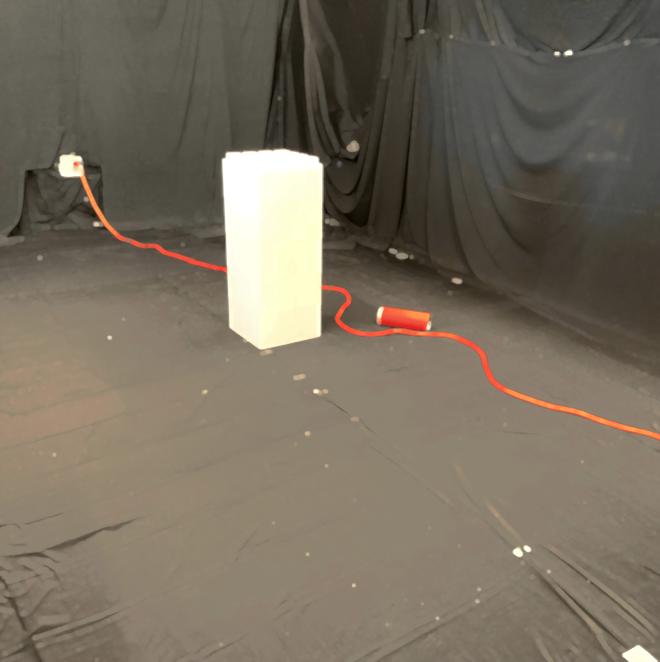
\includegraphics[width=80pt]{figures/teaser_knocking_end.png}};
\node [below=12pt of ws] (we) {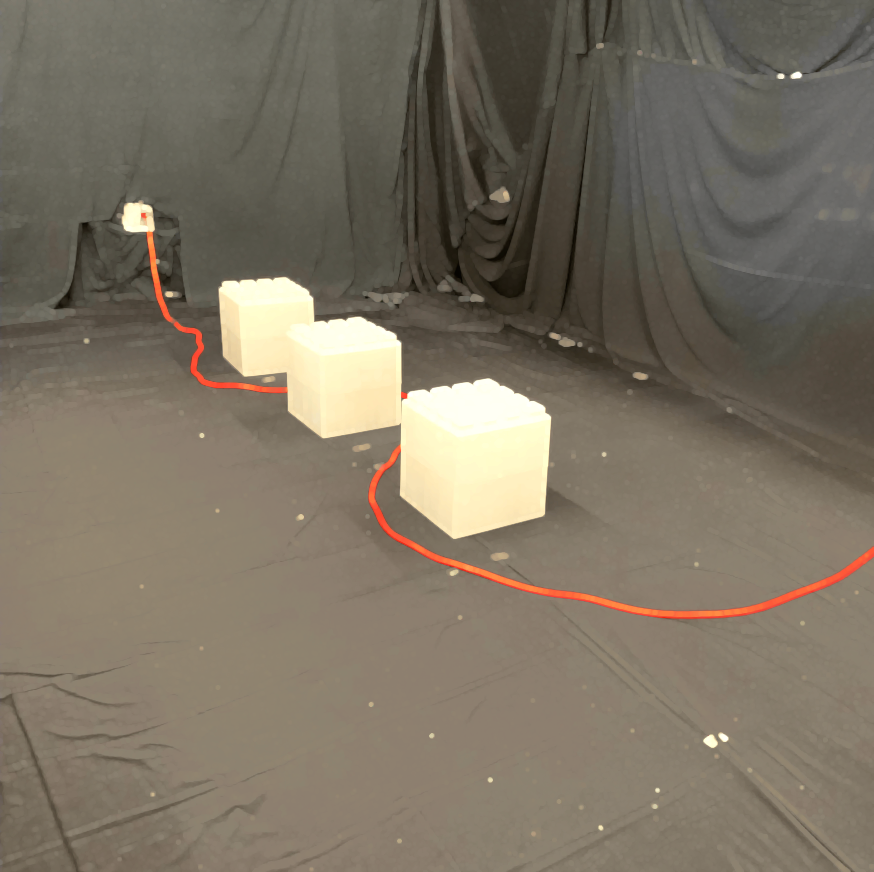
\includegraphics[width=80pt]{figures/teaser_weaving_end.png}};
\draw [arr] (vs) -- (ve);
\draw [arr] (ks) -- (ke);
\draw [arr] (ws) -- (we);
\node [below=4pt of ve] {\footnotesize (a) Task 1: Vaulting};
\node [below=4pt of ke] {\footnotesize (b) Task 2: Knocking};
\node [below=4pt of we] {\footnotesize (c) Task 3: Weaving};
\end{tikzpicture}
\caption{
\small
Illustration of the 3 tasks: Vaulting, Knocking, and Weaving in real experiments with an orange 18-gauge cable. %The cable is plugged into the wall on one end, and attached to the robot's gripper on the other end.
}
\vspace*{-15pt}
\label{fig:three_tasks}
\end{figure}